\documentclass[12pt]{article}

\usepackage[utf8]{inputenc}
\usepackage{amsmath,amssymb,hyperref,array,xcolor,multicol,verbatim,mathpazo}
\usepackage[normalem]{ulem}
\usepackage[pdftex]{graphicx}
\usepackage{fullpage}

\usepackage{threeparttable}
\usepackage{geometry}
\usepackage[format=hang,font=normalsize,labelfont=bf]{caption}
\usepackage{lscape}
\usepackage{natbib}
\usepackage{setspace}
\usepackage{float,color}
\usepackage[pdftex]{graphicx}
\usepackage{pdfsync}
\usepackage{placeins}
\usepackage{geometry}
\usepackage{pdflscape}
\usepackage[normalem]{ulem}
\usepackage{threeparttable, multirow}
\useunder{\uline}{\ul}{}
\synctex=1
\usepackage{hyperref}
\hypersetup{colorlinks,linkcolor=red,urlcolor=blue,citecolor=blue}
\usepackage{bm}


\newcommand{\E}{\mathbb{E}}

% Identifying information
\title{
Homework 4
} 
\author{Linghui Wu}
\date{\today}

\begin{document}

\maketitle

\section{Productivity Shocks in the Three Equation Model}

\subsection*{(a)}

Firstly, from 
\begin{align*}
\hat{a}_{t} &= \rho_{a} \hat{a}_{t-1} + \varepsilon_{t},
\end{align*}
we have 
\begin{align*}
\E_{t}\left[\hat{a}_{t+1}\right] &= \rho_{a}\hat{a}_{t}.
\end{align*}
The system of equations that characterizes the log-linearized NK model is
\begin{equation}
\label{eq:y_t}
\hat{y}_{t} = -\sigma\left(\hat{i}_{t}-\E_{t}\left[\hat{\pi}_{t}\right]\right) + \E_{t}\left[\hat{y}_{t+1}\right]
\end{equation}
\begin{equation}
\label{eq:pi_t}
\hat{\pi}_{t} = \kappa \left(\hat{y}_{t}-\frac{1+\phi}{\gamma+\phi}\hat{a}_{t}\right) + \beta\E_{t}\left[\hat{\pi}_{t+1}\right]
\end{equation}
\begin{equation}
\label{eq:i_t}
\hat{i}_{t} = \phi_{\pi}\hat{\pi}_{t}
\end{equation}
Using the method of undetermined coefficients, we assume that 
\begin{align*}
\hat{y}_{t} &= \eta_{ya}\hat{a}_{t} \\
\hat{\pi}_{t} &= \eta_{\pi a}\hat{a}_{t} \\
\hat{i}_{t} &= \eta_{ia}\hat{a}_{t}
\end{align*}
By simple algebra, equations (\ref{eq:y_t}), (\ref{eq:pi_t}) and (\ref{eq:i_t}) can be re-arranged as 
\begin{equation}
\label{eq:eta_ya}
\eta_{ya} = \frac{\sigma \left(\eta_{\pi a}\rho_{a}-\eta_{ia}\right)}{1-\rho_{a}}
\end{equation}
\begin{equation}
\label{eq:eta_pia}
\eta_{\pi a} = \frac{\kappa\left(\eta_{ya} - \frac{1+\varphi}{\gamma+\varphi}\right)}{1-\beta\rho_{a}}
\end{equation}
\begin{equation}
\label{eq:eta_ia}
\eta_{ia} = \phi_{\pi}\eta_{\pi a}
\end{equation}
Combining equations (\ref{eq:eta_ya}), (\ref{eq:eta_pia}) and (\ref{eq:eta_ia}),
we can pin down the three unknown coefficients
\newcommand{\etapia}{\frac{\kappa\left(1-\rho_{a}\right)\left(1+\varphi\right)}{\left(\gamma+\varphi\right)\left[\kappa\sigma\left(\rho_{a}-\phi_{\pi}\right)-\left(1-\rho_{a}\right)\left(1-\beta\rho_{a}\right)\right]}}
\begin{align*}
\eta_{ya} &= \frac{\sigma\left(\rho_{a}-\phi_{\pi}\right)}{1-\rho_{a}} \etapia \\
\eta_{\pi a} &= \etapia \\
\eta_{ia} &= \phi_{\pi}\etapia 
\end{align*}
Therefore, 
\begin{align*}
\hat{y}_{t} &= \frac{\sigma\left(\rho_{a}-\phi_{\pi}\right)}{1-\rho_{a}} \etapia \hat{a}_{t} \\
\hat{\pi}_{t} &= \etapia \hat{a}_{t} \\
\hat{i}_{t} &= \phi_{\pi}\etapia \hat{a}_{t}
\end{align*}

\subsection*{(b)}

By Fisher equation that $\E_{t}\left[R_{t+1}\right]=\E_{t}\left[Q_{t}\frac{P_{t}}{P_{t+1}}\right]$, we can derive
\begin{align*}
\hat{r}_{t} &= \hat{i}_{t} - E_{t}\left[\hat{\pi}_{t+1}\right] = \hat{i}_{t} - \eta_{\pi a}\rho_{a}\hat{a}_{t},
\end{align*}
and
\begin{align*}
\E_{t}\left[\hat{r}_{t+1}\right] &= \rho_{a}\left(\eta_{ia} - \eta_{\pi a}\rho_{a}\right) \hat{a}_{t}.
\end{align*}

\subsection*{(c)}

Figure \ref{fig:irf} plots the impulse response functions.
If the firm can frictionlessly adjust the price,
an increase in productivity will result in an equal rise in output. 
However, due to the nominal rigidities, 
the actual increase in production is smaller, 
leading to a negative output gap. 
This causes the firm's marginal costs to decrease, allowing it to lower the price and, in turn, the inflation rate reduces. 
The central bank lowers the nominal interest rate when the inflation rate decreases, 
leading to a reduction in the real interest rate as well.
Moreover, due to the price stickiness, the firm hires less labor to meet the demand, and the employment drops. 

\begin{figure}[ht]
\centering
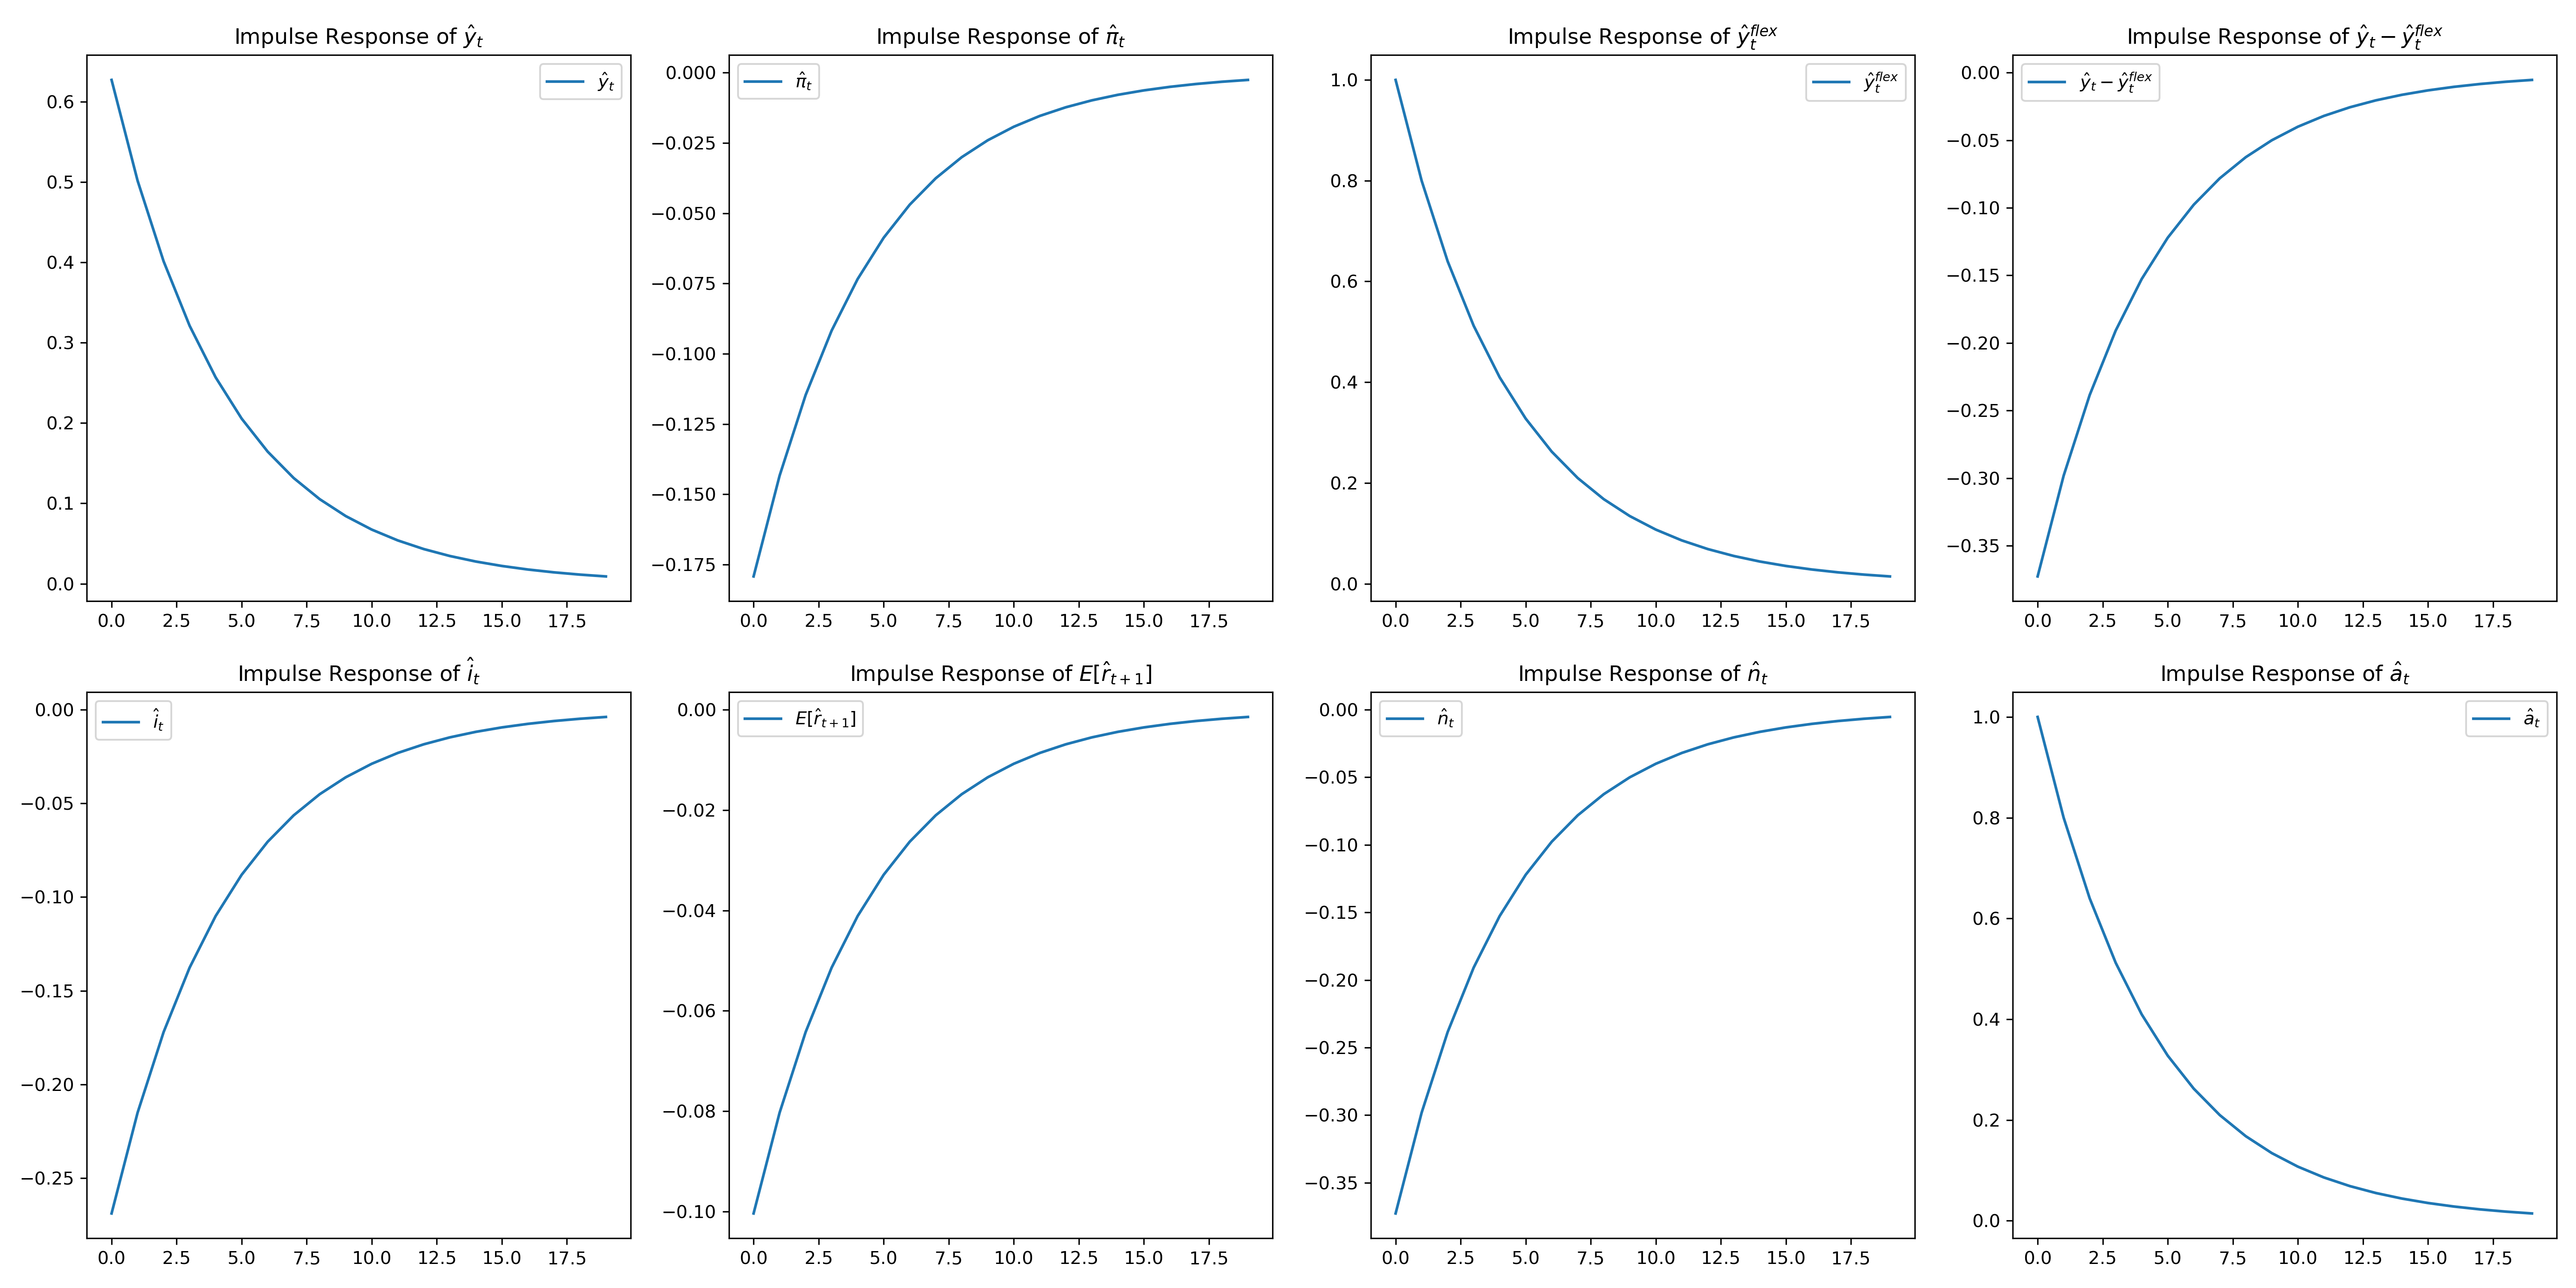
\includegraphics[width=0.8\textwidth]{figs/q1_IRFs.png}
\caption{Impulse Response Functions}
\label{fig:irf}
\end{figure}

\subsection*{(d)}

The impulse responses in figure \ref{fig:irf} are comparable to those in \texttt{newkeysianlinear.ipynb}.

\section{Non-linear NK Model in Jupyter}

\subsection*{(a)}

Mathematically, this expression is not recursive because it does not contain $P^{\ast}_{t+s} \forall s \in \mathbb{N}$. 
This is because the objective function for the intermediate producer's optimal reset pricing 
only puts weight on states of the world in which the price they set remains $P^{\ast}_{t}$ forever. 

Intuitively, when a firm gets to reset its price, its history does not matter,
which indicates that previous price-setting decisions do not affect future reset prices. 

\subsection*{(b)}

We are given 
\begin{equation}
\label{eq:lambda}
\Lambda_{t,t+k} = \Lambda_{t,t+1}\Lambda_{t+1,t+k} \forall
\end{equation}
\begin{equation}
\label{eq:F2}
F_{2,t} = \Sigma^{\infty}_{k=0}\theta^{k}\Lambda_{t,t+k}Y_{t+k}\left(\frac{P_{t+k}}{P_{t}}\right)^{\epsilon-1}.
\end{equation}
Iterating forward equation (\ref{eq:F2}) by one period, we have
\begin{equation}
\label{eq:F2prime}
F_{2,t+1} = \Sigma^{\infty}_{k=0}\theta^{k}\Lambda_{t+1,t+k+1}Y_{t+k+1}\left(\frac{P_{t+k+1}}{P_{t+1}}\right)^{\epsilon-1}.
\end{equation}
So,
\begin{align*}
F_{2,t} &= \theta^{0}\Lambda_{t,t}Y_{t} + \Sigma^{\infty}_{k=1} \theta^{k}\Lambda_{t,t+k}Y_{t+k}\left(\frac{P_{t+k}}{P_{t}}\right)^{\epsilon-1} \\
&= Y_{t} + \Sigma^{\infty}_{k=0} \theta^{k+1}\Lambda_{t,t+k+1}Y_{t+k+1}\left(\frac{P_{t+k+1}}{P_{t}}\right)^{\epsilon-1} \\
&= Y_{t} + \theta \Sigma^{\infty}_{k=0} \theta^{k}\Lambda_{t,t+1}\Lambda_{t+1,t+k}Y_{t+k+1}\left(\frac{P_{t+k+1}}{P_{t+1}}\frac{P_{t+1}}{P_{t}}\right)^{\epsilon-1} \\
&= Y_{t} + \theta\left(\Pi_{t+1}\right)^{\epsilon-1}\Lambda_{t,t+1}F_{2,t+1}.
\end{align*}

\subsection*{(c)}

By a similar argument as in part (b), we have
\begin{align*}
\label{eq:F1}
F_{1,t} &=\left(1+\mu\right)\Sigma^{\infty}_{s=0}\theta^{s}\Lambda_{t,t+s}Y_{t+s}\left(\frac{P_{t+s}}{P_{t}}\right)^{\epsilon-1}\frac{W_{t+s}}{P_{t}A_{t+s}} \\
&= \left(1+\mu\right)Y_{t}\frac{W_{t}}{P_{t}A_{t}} + \left(1+\mu\right)\Sigma^{\infty}_{s=1}\theta^{s}\Lambda_{t,t+s}Y_{t+s}\left(\frac{P_{t+s}}{P_{t}}\right)^{\epsilon-1}\frac{W_{t+s}}{P_{t}A_{t+s}} \\
&= \left(1+\mu\right)Y_{t}\frac{W_{t}}{P_{t}A_{t}} + \left(1+\mu\right)\Sigma^{\infty}_{s=0}\theta^{s+1}\Lambda_{t,t+1}\Lambda_{t+1,t+s+1}\left(\frac{P_{t+s+1}}{P_{t+1}}\frac{P_{t+1}}{P_{t}}\right)^{\epsilon-1}\frac{W_{t+s+1}}{P_{t}A_{t+s+1}}\frac{P_{t+1}}{P_{t+1}} \\
&= \left(1+\mu\right)Y_{t}\frac{W_{t}}{P_{t}A_{t}} + \theta\left(\Pi_{t+1}\right)^{\epsilon}\Lambda_{t,t+1}F_{1,t+1}.
\end{align*}

\subsection*{(d)}

By definition, 
\begin{equation}
\label{eq:pi}
\Pi_{t} = \frac{P_{t}}{P_{t-1}},
\end{equation} 
and
\begin{equation}
\label{eq:reset_p}
P_{t} = \left[\theta P^{1-\epsilon}_{t-1} + \left(1-\theta\right)P^{\ast}_{t}\right]^{\frac{1}{1-\epsilon}}.
\end{equation}
Dividing both sides of equation (\ref{eq:reset_p}) by $P^{1-\epsilon}_{t}$ and rearranging yields the desired result,
\begin{align*}
1 = \theta\left(\Pi_{t}\right)^{\epsilon-1}+\left(1-\theta\right)\left(p^{\ast}_{t}\right)^{1-\epsilon}.
\end{align*}

\subsection*{(e)}

If $p^{\ast}_{t} > 1$, it means that the reset price is higher than the current price. 
For equation (\ref{eq:reset_p}) to hold, we need $P_{t}^{\ast} > P_{t} > P_{t+1}$, which implies that $\Pi_{t}=\frac{P_{t}}{P_{t-1}} > 1$.
Intuitively, $p^{\ast}_{t} > 1$ implies that the optimal reset price at time $t$ is very high relative to the current price. 
If the firm can flexibly adjust the prices, the firm will significantly increase the price, 
indicating that the current inflation must also be high since the prices are going up.

\subsection*{(f)-(g)}

\subsection*{(h)}

\subsection*{(i)}

\end{document}


